\documentclass[
  shownotes,
  xcolor={svgnames},
  hyperref={colorlinks,citecolor=DarkBlue,linkcolor=DarkRed,urlcolor=DarkBlue}
  , aspectratio=169]{beamer}
\usepackage{animate}
\usepackage{amsmath}
\usepackage{amsfonts}
\usepackage{amssymb}
\usepackage{pifont}
\usepackage{mathpazo}
%\usepackage{xcolor}
\usepackage{multimedia}
\usepackage{fancybox}
\usepackage[para]{threeparttable}
\usepackage{multirow}
\setcounter{MaxMatrixCols}{30}
\usepackage{subcaption}
\usepackage{graphicx}
\usepackage{lscape}
\usepackage[compatibility=false,font=small]{caption}
\usepackage{booktabs}
\usepackage{ragged2e}
\usepackage{chronosys}
\usepackage{appendixnumberbeamer}
\usepackage{animate}
\setbeamertemplate{caption}[numbered]
\usepackage{color}
%\usepackage{times}
\usepackage{tikz}
\usepackage{comment} %to comment
%% BibTeX settings
\usepackage{natbib}
\bibliographystyle{apalike}
\bibpunct{(}{)}{,}{a}{,}{,}
\setbeamertemplate{bibliography item}{[\theenumiv]}

% Defines columns for bespoke tables
\usepackage{array}
\newcolumntype{L}[1]{>{\raggedright\let\newline\\\arraybackslash\hspace{0pt}}m{#1}}
\newcolumntype{C}[1]{>{\centering\let\newline\\\arraybackslash\hspace{0pt}}m{#1}}
\newcolumntype{R}[1]{>{\raggedleft\let\newline\\\arraybackslash\hspace{0pt}}m{#1}}


\usepackage{xfrac}


\usepackage{multicol}
\setlength{\columnsep}{0.5cm}

% Theme and colors
\usetheme{Boadilla}

% I use steel blue and a custom color palette. This defines it.
\definecolor{andesred}{HTML}{af2433}

% Other options
\providecommand{\U}[1]{\protect\rule{.1in}{.1in}}
\usefonttheme{serif}
\setbeamertemplate{itemize items}[default]
\setbeamertemplate{enumerate items}[square]
\setbeamertemplate{section in toc}[circle]

\makeatletter

\definecolor{mybackground}{HTML}{82CAFA}
\definecolor{myforeground}{HTML}{0000A0}

\setbeamercolor{normal text}{fg=black,bg=white}
\setbeamercolor{alerted text}{fg=red}
\setbeamercolor{example text}{fg=black}

\setbeamercolor{background canvas}{fg=myforeground, bg=white}
\setbeamercolor{background}{fg=myforeground, bg=mybackground}

\setbeamercolor{palette primary}{fg=black, bg=gray!30!white}
\setbeamercolor{palette secondary}{fg=black, bg=gray!20!white}
\setbeamercolor{palette tertiary}{fg=white, bg=andesred}

\setbeamercolor{frametitle}{fg=andesred}
\setbeamercolor{title}{fg=andesred}
\setbeamercolor{block title}{fg=andesred}
\setbeamercolor{itemize item}{fg=andesred}
\setbeamercolor{itemize subitem}{fg=andesred}
\setbeamercolor{itemize subsubitem}{fg=andesred}
\setbeamercolor{enumerate item}{fg=andesred}
\setbeamercolor{item projected}{bg=gray!30!white,fg=andesred}
\setbeamercolor{enumerate subitem}{fg=andesred}
\setbeamercolor{section number projected}{bg=gray!30!white,fg=andesred}
\setbeamercolor{section in toc}{fg=andesred}
\setbeamercolor{caption name}{fg=andesred}
\setbeamercolor{button}{bg=gray!30!white,fg=andesred}



\usepackage{fancyvrb}
\newcommand{\VerbBar}{|}
\newcommand{\VERB}{\Verb[commandchars=\\\{\}]}
\DefineVerbatimEnvironment{Highlighting}{Verbatim}{commandchars=\\\{\}}
% Add ',fontsize=\small' for more characters per line
\usepackage{framed}
\definecolor{shadecolor}{RGB}{248,248,248}
\newenvironment{Shaded}{\begin{snugshade}}{\end{snugshade}}
\newcommand{\AlertTok}[1]{\textcolor[rgb]{0.94,0.16,0.16}{#1}}
\newcommand{\AnnotationTok}[1]{\textcolor[rgb]{0.56,0.35,0.01}{\textbf{\textit{#1}}}}
\newcommand{\AttributeTok}[1]{\textcolor[rgb]{0.77,0.63,0.00}{#1}}
\newcommand{\BaseNTok}[1]{\textcolor[rgb]{0.00,0.00,0.81}{#1}}
\newcommand{\BuiltInTok}[1]{#1}
\newcommand{\CharTok}[1]{\textcolor[rgb]{0.31,0.60,0.02}{#1}}
\newcommand{\CommentTok}[1]{\textcolor[rgb]{0.56,0.35,0.01}{\textit{#1}}}
\newcommand{\CommentVarTok}[1]{\textcolor[rgb]{0.56,0.35,0.01}{\textbf{\textit{#1}}}}
\newcommand{\ConstantTok}[1]{\textcolor[rgb]{0.00,0.00,0.00}{#1}}
\newcommand{\ControlFlowTok}[1]{\textcolor[rgb]{0.13,0.29,0.53}{\textbf{#1}}}
\newcommand{\DataTypeTok}[1]{\textcolor[rgb]{0.13,0.29,0.53}{#1}}
\newcommand{\DecValTok}[1]{\textcolor[rgb]{0.00,0.00,0.81}{#1}}
\newcommand{\DocumentationTok}[1]{\textcolor[rgb]{0.56,0.35,0.01}{\textbf{\textit{#1}}}}
\newcommand{\ErrorTok}[1]{\textcolor[rgb]{0.64,0.00,0.00}{\textbf{#1}}}
\newcommand{\ExtensionTok}[1]{#1}
\newcommand{\FloatTok}[1]{\textcolor[rgb]{0.00,0.00,0.81}{#1}}
\newcommand{\FunctionTok}[1]{\textcolor[rgb]{0.00,0.00,0.00}{#1}}
\newcommand{\ImportTok}[1]{#1}
\newcommand{\InformationTok}[1]{\textcolor[rgb]{0.56,0.35,0.01}{\textbf{\textit{#1}}}}
\newcommand{\KeywordTok}[1]{\textcolor[rgb]{0.13,0.29,0.53}{\textbf{#1}}}
\newcommand{\NormalTok}[1]{#1}
\newcommand{\OperatorTok}[1]{\textcolor[rgb]{0.81,0.36,0.00}{\textbf{#1}}}
\newcommand{\OtherTok}[1]{\textcolor[rgb]{0.56,0.35,0.01}{#1}}
\newcommand{\PreprocessorTok}[1]{\textcolor[rgb]{0.56,0.35,0.01}{\textit{#1}}}
\newcommand{\RegionMarkerTok}[1]{#1}
\newcommand{\SpecialCharTok}[1]{\textcolor[rgb]{0.00,0.00,0.00}{#1}}
\newcommand{\SpecialStringTok}[1]{\textcolor[rgb]{0.31,0.60,0.02}{#1}}
\newcommand{\StringTok}[1]{\textcolor[rgb]{0.31,0.60,0.02}{#1}}
\newcommand{\VariableTok}[1]{\textcolor[rgb]{0.00,0.00,0.00}{#1}}
\newcommand{\VerbatimStringTok}[1]{\textcolor[rgb]{0.31,0.60,0.02}{#1}}
\newcommand{\WarningTok}[1]{\textcolor[rgb]{0.56,0.35,0.01}{\textbf{\textit{#1}}}}
\usepackage{graphicx}
\makeatletter

\makeatother


%%%%%%%%%%%%%%% BEGINS DOCUMENT %%%%%%%%%%%%%%%%%%

\begin{document}

\title{Lecture 2:  Sobreajuste \&  Validación Cruzada}
\subtitle{Aprendizaje y Minería de Datos para los Negocios}
\date{\today}

\author[Sarmiento-Barbieri]{Ignacio Sarmiento-Barbieri}
\institute[Uniandes]{Universidad de los Andes}


\begin{frame}[noframenumbering]
\maketitle
\end{frame}

%%%%%%%%%%%%%%%%%%%%%%%%%%%%%%%%%%%
%       Motivation              %
% What is the question?
% Why do we care?
% What is new?
% What do you find?
%%%%%%%%%%%%%%%%%%%%%%%%%%%%%%%%%%%




\begin{frame}
\frametitle{Agenda}

\tableofcontents


\end{frame}
%----------------------------------------------------------------------%
\section{Recap}
%----------------------------------------------------------------------%
%----------------------------------------------------------------------%
\begin{frame}
\frametitle{Predicción y Error Predictivo}


\begin{itemize}
  \item El objetivo es predecir $Y$ dadas otras variables $X$. Ej: precio vivienda dadas las caracteristicas
  \bigskip
  \item Asumimos que el link entre $Y$ and $X$ esta dado por el modelo:
\end{itemize}
\bigskip
\begin{align}
  Y = f(X) + u
\end{align}
\bigskip
\begin{itemize}
  \item donde $f(X)$ es cualquier funcion, 
  \bigskip
  \item  $u$ una variable aleatoria no observable $E(u)=0$ and $V(u) = \sigma^2$
\end{itemize}


\end{frame}

%----------------------------------------------------------------------%
\begin{frame}
\frametitle{Predicción y Error Predictivo}

\begin{itemize}
  \item En la práctica no conocemos $f(X)$
  \item Es necesario estimarla $\hat Y = \hat f(X)$ 

\end{itemize}

\medskip
Entonces
\begin{align}
  Err (  Y )  &= MSE(\hat f) + \sigma^2  \\
                 &= Bias^2(\hat f) + V(\hat f) +  Irreducible\,Error
\end{align}
\medskip
Dos partes 
\begin{itemize}
  \item  el error de estimar $f$ con $\hat f$. (\emph{reducible})
  \item  el error de no observar $u$. (\emph{irreducible})
\end{itemize}

\medskip

Este resultado es muy importante,  
\begin{itemize}
\item predecir $Y$ implica predecir bien $f$.
\item existe un dilema entre sesgo y varianza
\end{itemize}

\end{frame}
%----------------------------------------------------------------------%
\section{Overfit}
%----------------------------------------------------------------------%
\begin{frame}[fragile]
\frametitle{Overfit}


        \begin{figure}[H] \centering
            \captionsetup{justification=centering}
              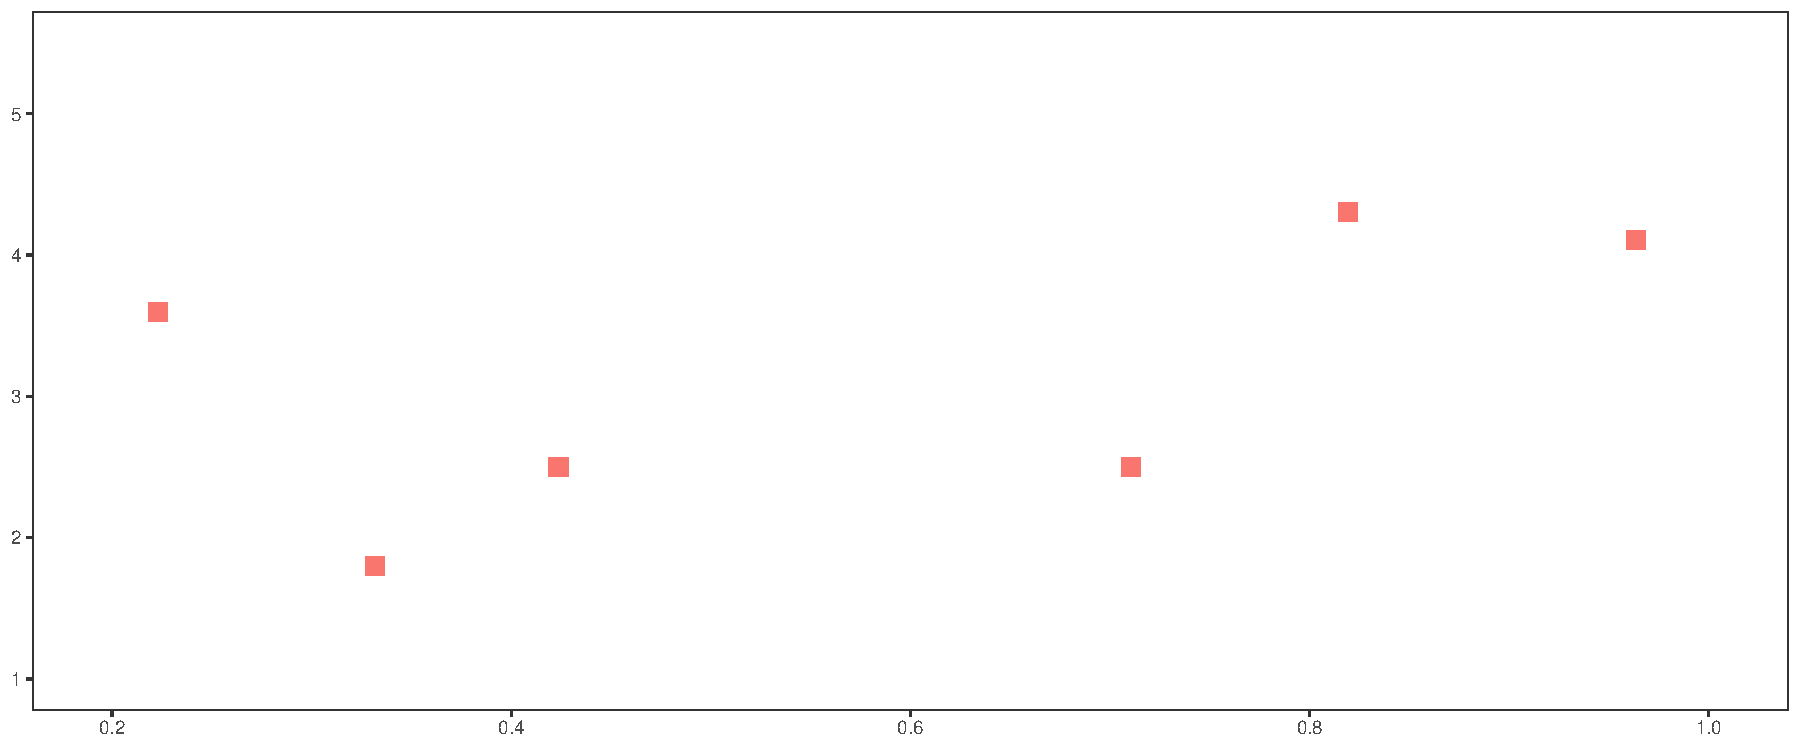
\includegraphics[scale=0.4]{figures/fig_1a.pdf}
 \end{figure}

\end{frame}

%----------------------------------------------------------------------%
\begin{frame}[fragile, noframenumbering]
\frametitle{Overfit}


        \begin{figure}[H] \centering
            \captionsetup{justification=centering}
              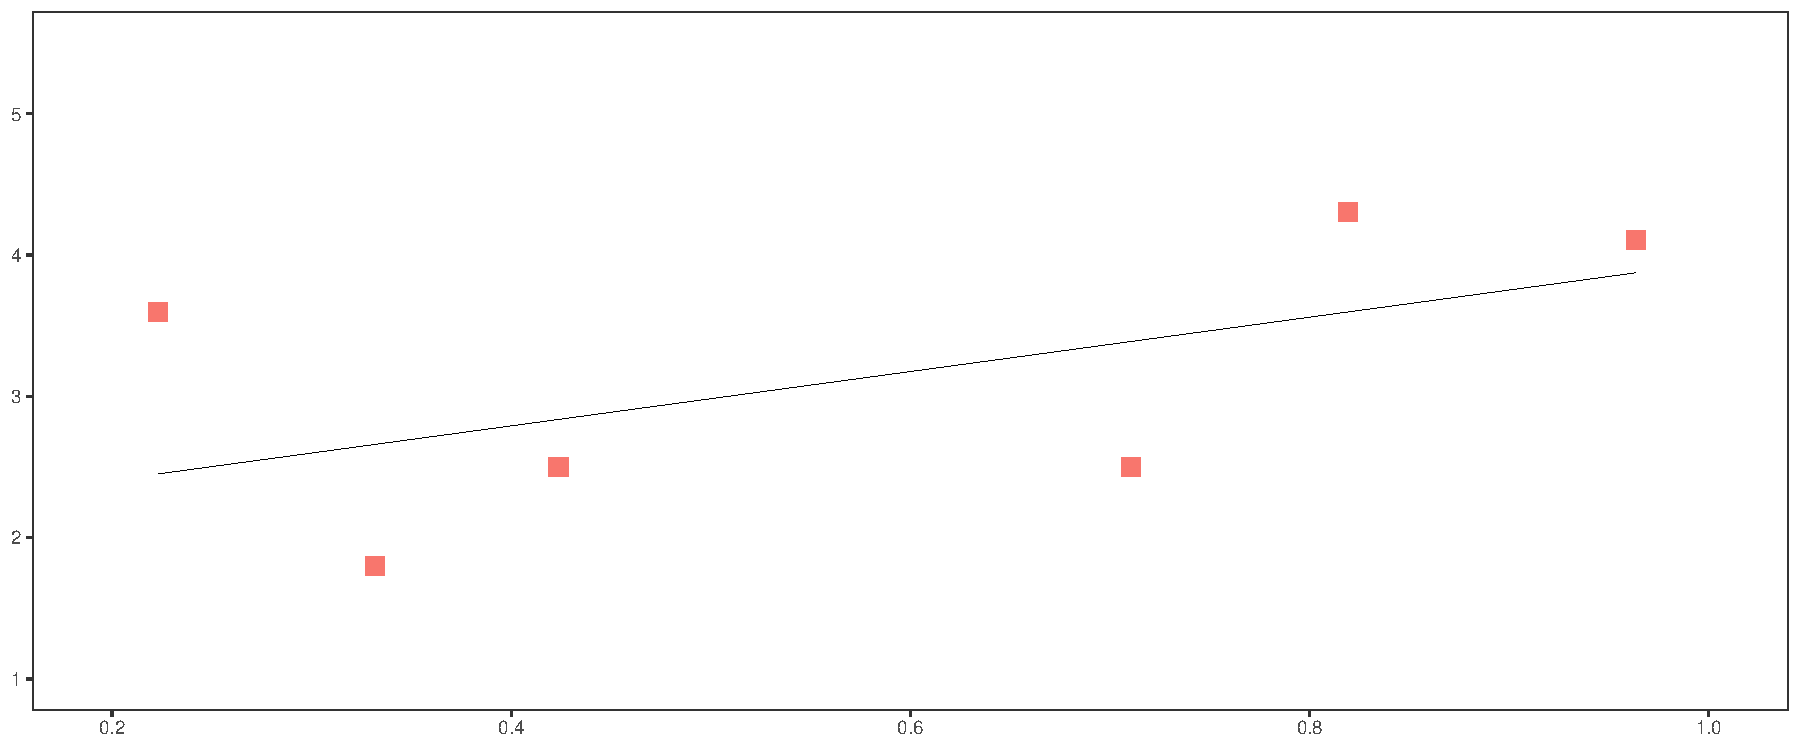
\includegraphics[scale=0.4]{figures/fig_1b.pdf}
 \end{figure}

\end{frame}
%----------------------------------------------------------------------%
\begin{frame}[fragile, noframenumbering]
\frametitle{Overfit}


        \begin{figure}[H] \centering
            \captionsetup{justification=centering}
              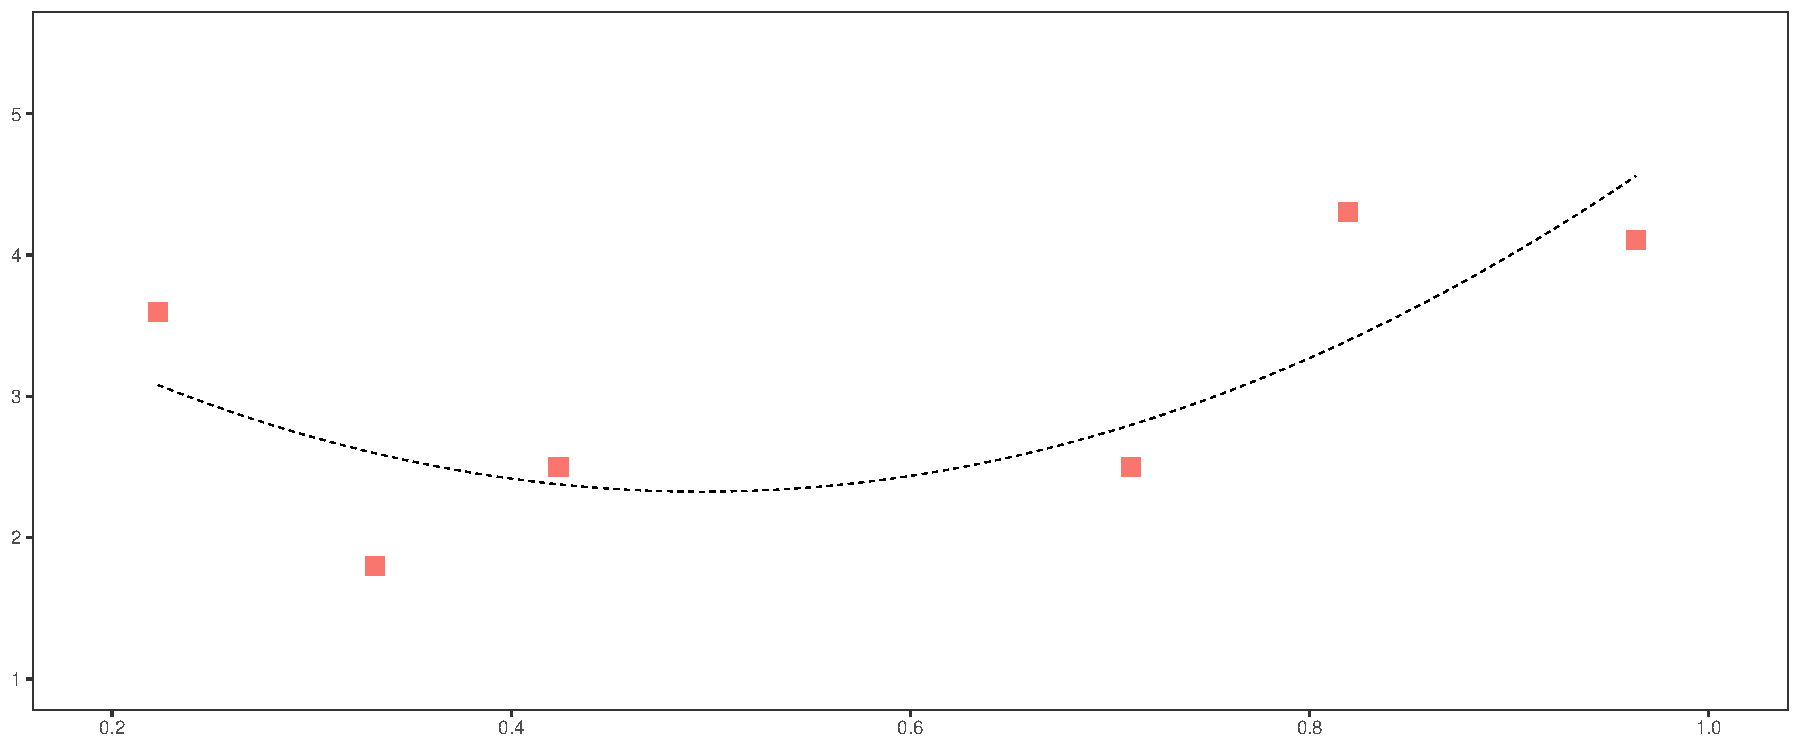
\includegraphics[scale=0.4]{figures/fig_1c.pdf}
 \end{figure}

\end{frame}

%----------------------------------------------------------------------%
\begin{frame}[fragile, noframenumbering]
\frametitle{Overfit}


        \begin{figure}[H] \centering
            \captionsetup{justification=centering}
              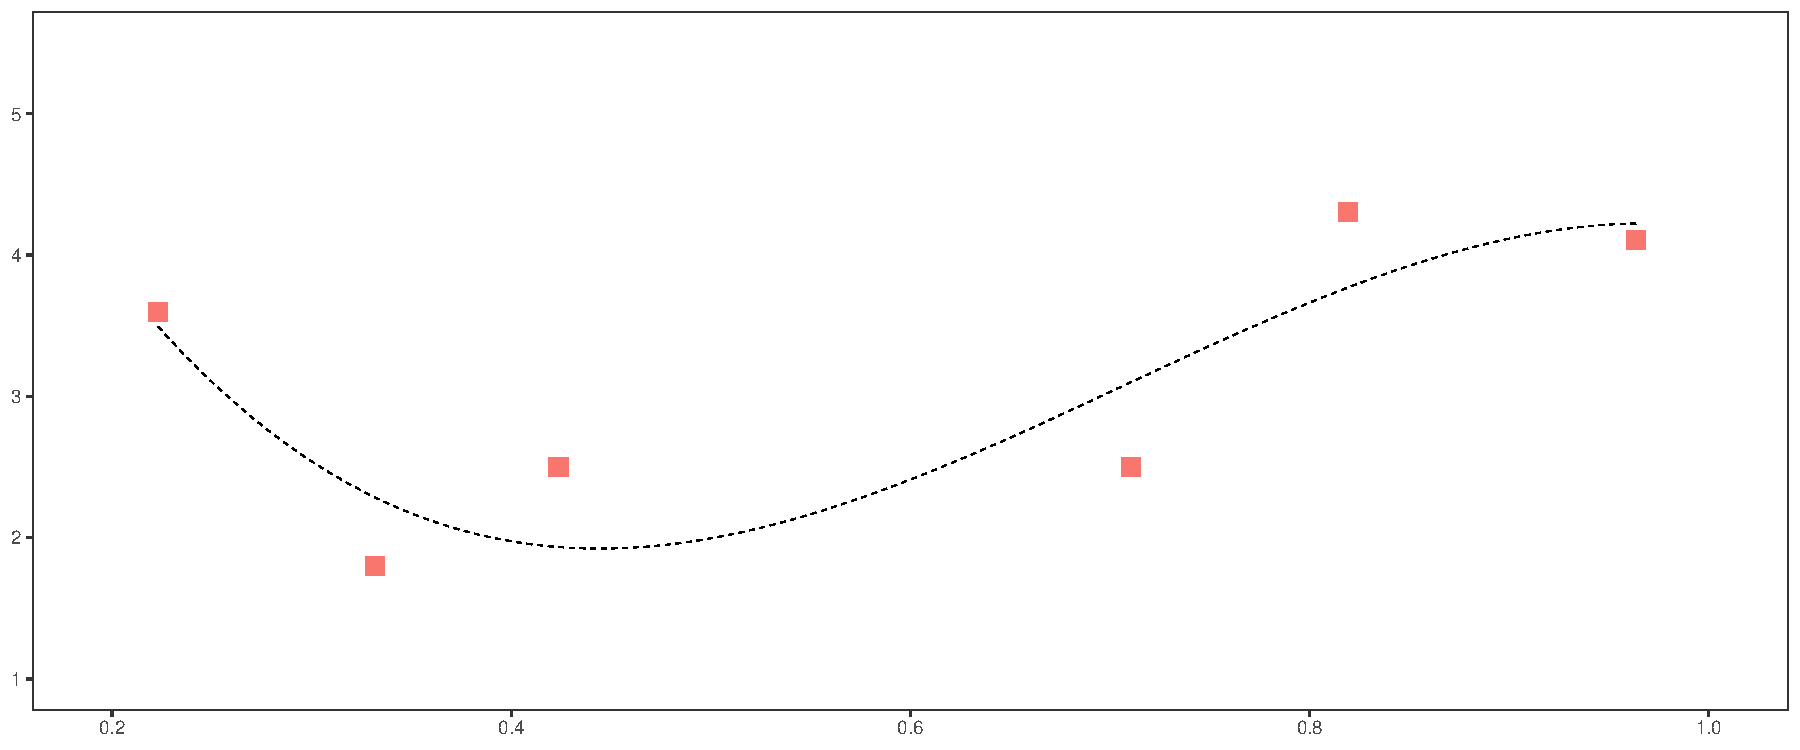
\includegraphics[scale=0.4]{figures/fig_1d.pdf}
 \end{figure}

\end{frame}
%----------------------------------------------------------------------%
\begin{frame}[fragile, noframenumbering]
\frametitle{Overfit}


        \begin{figure}[H] \centering
            \captionsetup{justification=centering}
              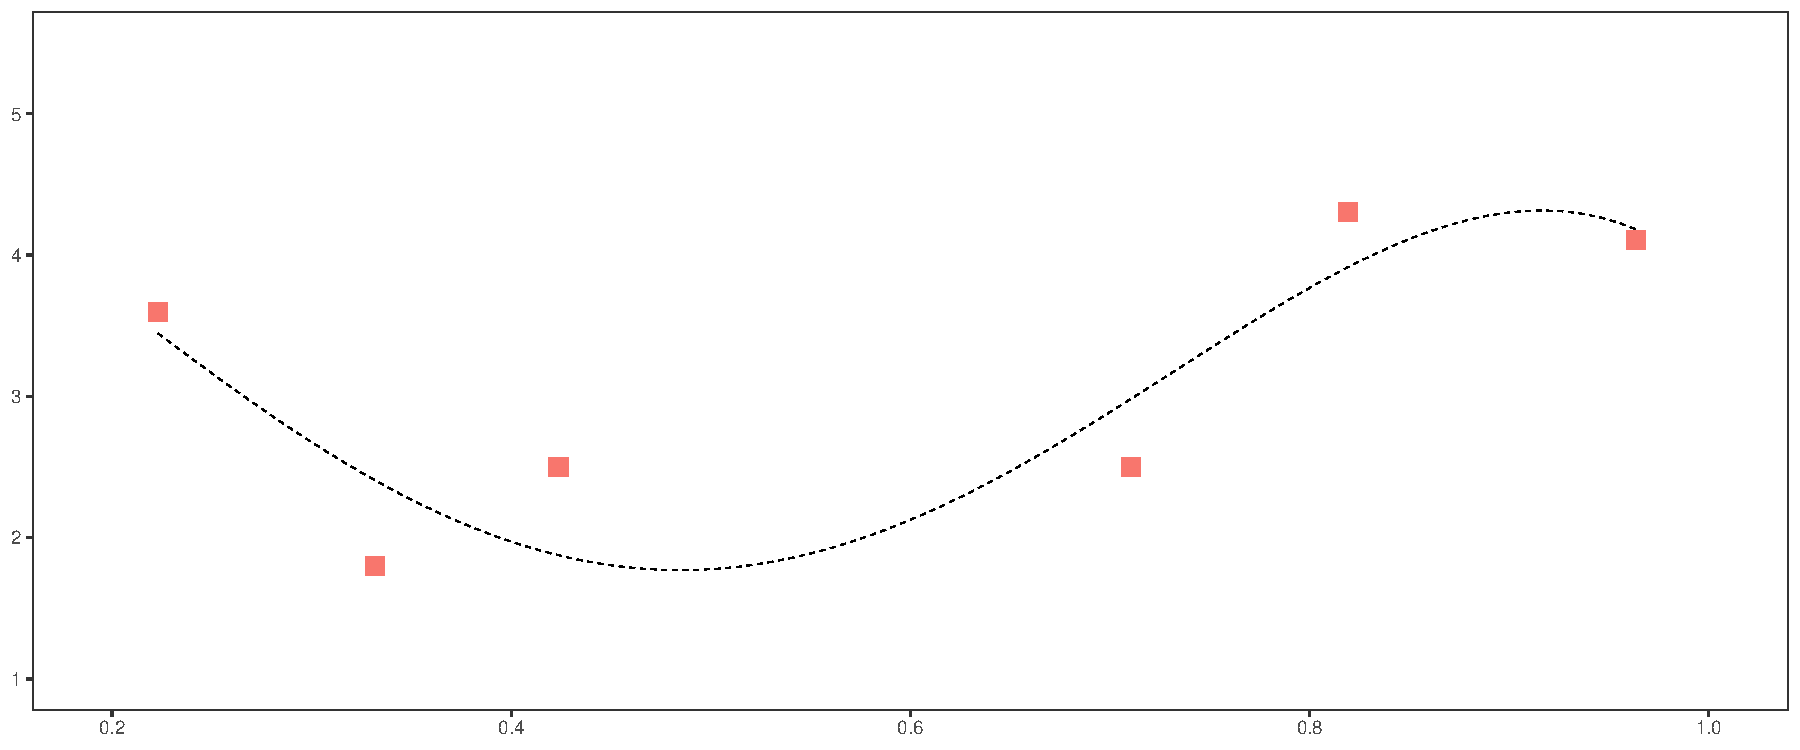
\includegraphics[scale=0.4]{figures/fig_1e.pdf}
 \end{figure}

\end{frame}
%----------------------------------------------------------------------%
\begin{frame}[fragile, noframenumbering]
\frametitle{Overfit}


        \begin{figure}[H] \centering
            \captionsetup{justification=centering}
              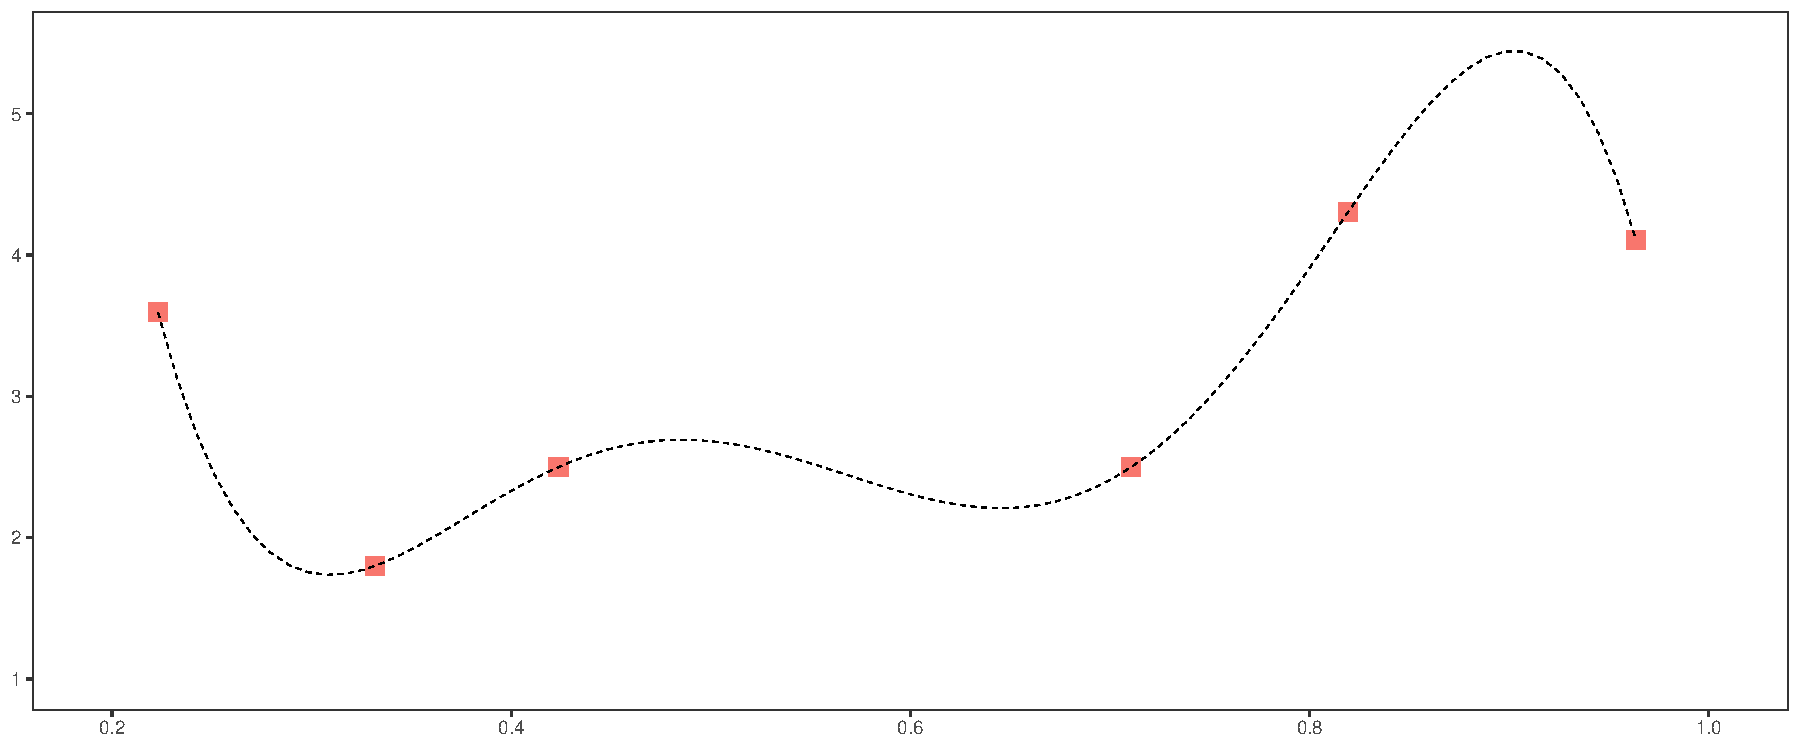
\includegraphics[scale=0.4]{figures/fig_1f.pdf}
 \end{figure}

\end{frame}
%----------------------------------------------------------------------%
\begin{frame}[fragile, noframenumbering]
\frametitle{Overfit}


        \begin{figure}[H] \centering
            \captionsetup{justification=centering}
              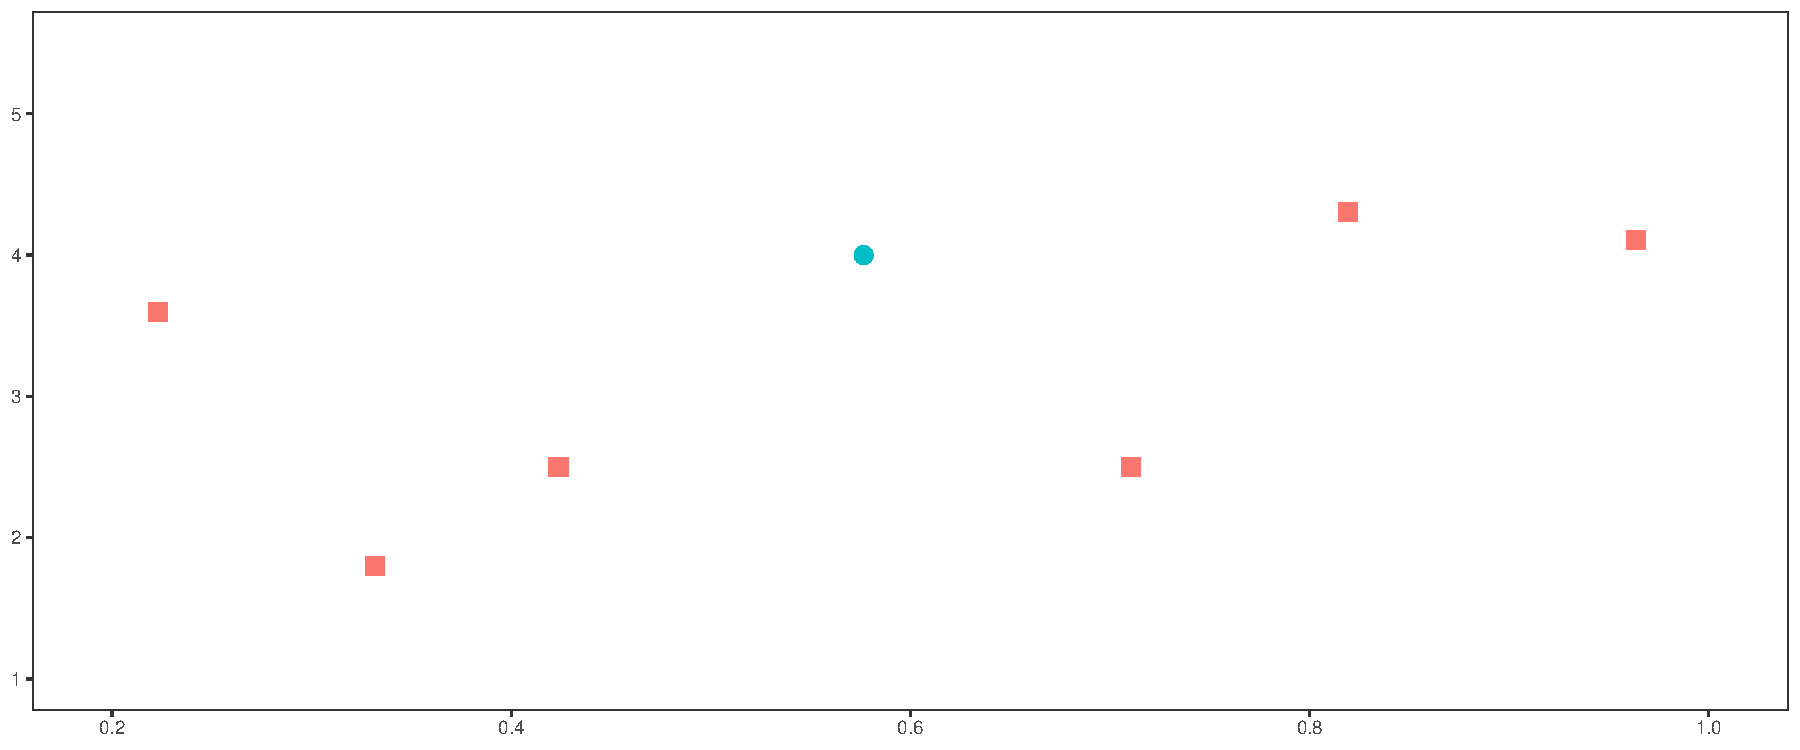
\includegraphics[scale=0.4]{figures/fig_1g.pdf}
 \end{figure}

\end{frame}
%----------------------------------------------------------------------%
\begin{frame}[fragile, noframenumbering]
\frametitle{Overfit}


        \begin{figure}[H] \centering
            \captionsetup{justification=centering}
              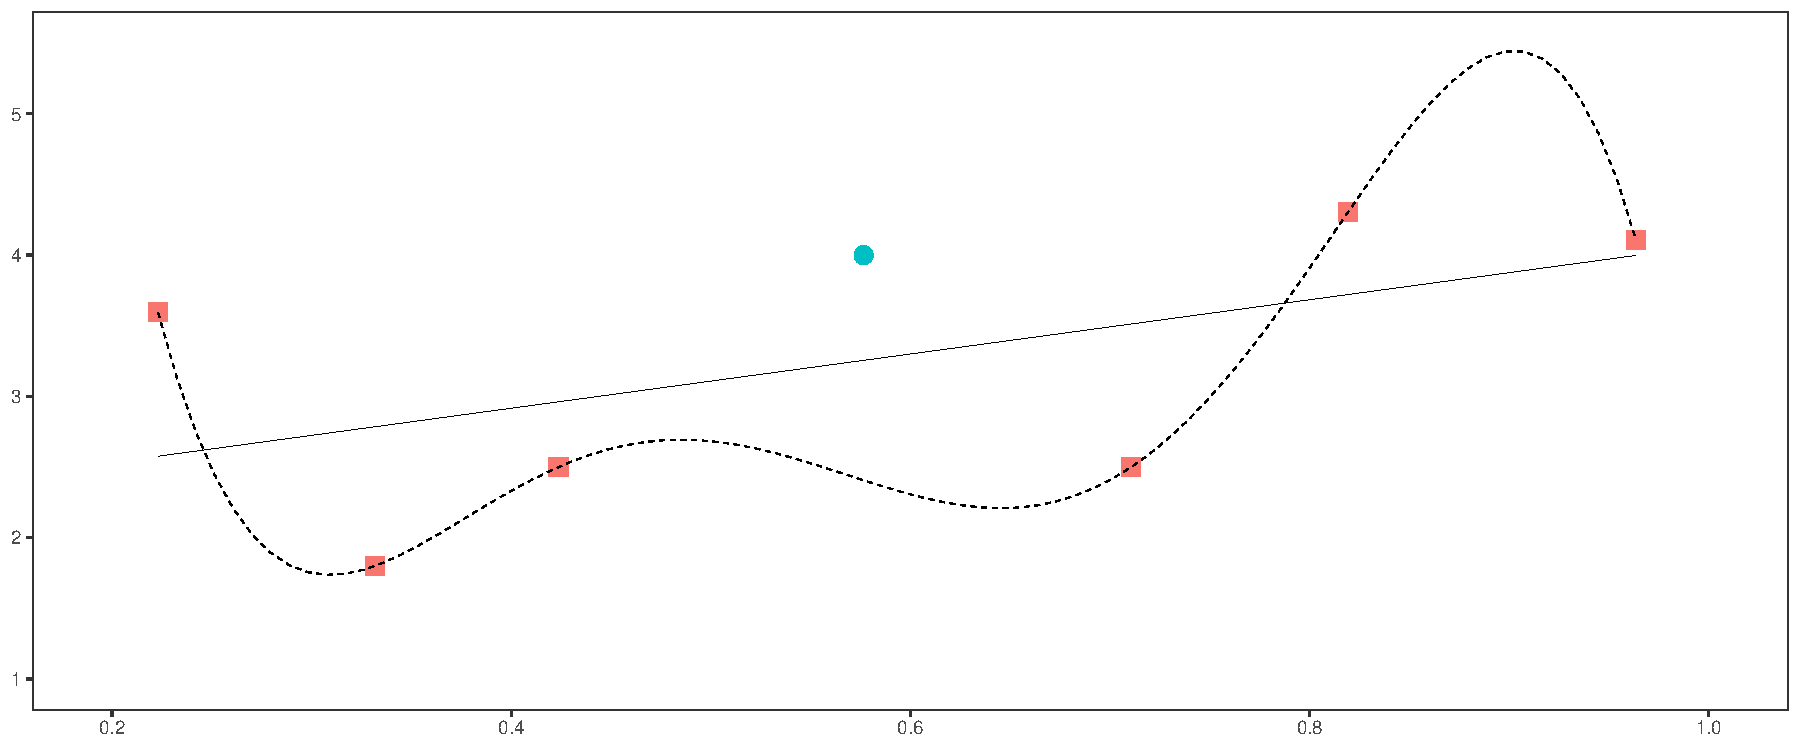
\includegraphics[scale=0.4]{figures/fig_1h.pdf}
 \end{figure}

\end{frame}
%----------------------------------------------------------------------%
\begin{frame}[fragile]
\frametitle{Overfit}


\begin{itemize}

  \item En efecto si el modelo verdadero es $y=f(x) +u$ 
  \medskip
  \item donde $f$ es un polinomio de grado $p^*$, with $E(u)=0$ and $V(u)=\sigma^2$
  \medskip
  \item con $p^*$ finito pero desconocido
  \medskip
  \item  podemos ajustar polinomios de grados crecientes $p=1,2,....$
  
  \begin{align}
  Err (  Y )  &= MSE(\hat f) + \sigma^2  \\
                 &= Bias^2(\hat f) + V(\hat f)  + Irreducible\,Error        
  \end{align}

  
\end{itemize}

\end{frame}
%----------------------------------------------------------------------%
\begin{frame}[fragile]
\frametitle{Overfit}


\begin{itemize}

  \item Bias ?

\end{itemize}

  \begin{align}
  \hat f(x) = X'\hat\beta=\sum_{s=0}^p x^s\hat\beta_s = x'\hat\beta  
  \end{align}

  donde $X'=(1,x,,x^2,\dots,x^p)$



\end{frame}
%----------------------------------------------------------------------%
\begin{frame}[fragile]
\frametitle{Overfit}


\begin{itemize}

  \item Varianza:
\end{itemize}

 
  \begin{align}
  V(\hat f(x) ) = V(X'\hat\beta) = \sigma^2 \frac{p}{n}
  \end{align}

 

Después de  $p^*$ aumentar la complejidad no reduce el sesgo, pero la varianza aumenta monotónicamente para  $\sigma^2$ y $n$ dados
 
\end{frame}
%----------------------------------------------------------------------%
\subsection{Overfit y Predicción fuera de Muestra}
%----------------------------------------------------------------------%
\begin{frame}[fragile]
\frametitle{Overfit y Predicción fuera de Muestra}


\begin{itemize}
  \item ML nos interesa la predicción fuera de muestra
  \medskip
  \item Overfit: modelos complejos predicen muy bien dentro de muestra, pero tienden a hacer un trabajo fuera de muestra 
  \medskip
  \item Hay que elegir el nivel adecuado de complejidad 
  \medskip
  \item Como medimos el error de predicción fuera de muestra?
  \medskip
  \item $R^2$ no funciona: mide predicción dentro de muestra, es no decreciente en complejidad
\end{itemize}


\end{frame}
%----------------------------------------------------------------------%
\begin{frame}[fragile]
\frametitle{Overfit y Predicción fuera de Muestra}


\begin{itemize}

\item Dos conceptos importantes
\medskip
\begin{itemize}
  \item {\it Test Error}: es el error de predicción en la muestra de prueba (test)
  \medskip
  \begin{align}
    Err_{\mathcal{T}est} =MSE[(Y,\hat Y)|\mathcal{T}est]
  \end{align}
  \medskip
  \item {\it Training error}:es el error de predicción en la muestra de entrenamiento (training)
  \medskip
  \begin{align}
    Err_{\mathcal{T}rain} = MSE[(Y,\hat Y)|\mathcal{T}rain]
  \end{align}
    \end{itemize}
    \medskip
  \item Como elegimos $\mathcal{T}est$?
  
\end{itemize}



\end{frame}
%----------------------------------------------------------------------%
\section{ Métodos de Remuestreo}
%----------------------------------------------------------------------%
\begin{frame}[fragile]
\frametitle{Qué son los Métodos de Remuestreo?}

\begin{itemize}



\item Herramientas que implican extraer repetidamente muestras de un conjunto de entrenamiento y reajustar el modelo de interés en cada muestra para obtener más información sobre el modelo.
\medskip
\item Evaluación del modelo: estimar el error de predicción en la muestra de prueba
\medskip
\item Selección de modelo: seleccione el nivel apropiado de flexibilidad del modelo
\medskip
\item ¡Son computacionalmente costosos! Pero en estos días tenemos computadoras poderosas

\end{itemize}




\end{frame}
%----------------------------------------------------------------------%
\subsection{Enfoque de conjunto de validación}
%----------------------------------------------------------------------%
\begin{frame}[fragile]
\frametitle{Enfoque de conjunto de validación}

\begin{itemize}
\item Suponga que nos gustaría encontrar un conjunto de variables que den el menor  error de predicción en la muestra de prueba (no de entrenamiento) 
\item Si tenemos muchos datos, podemos lograr este objetivo dividiendo aleatoriamente los datos en partes de entrenamiento y validación (prueba)
\item Luego usaríamos la parte de entrenamiento para construir cada modelo posible (es decir, las diferentes combinaciones de variables) y elegimos el modelo que dio lel menor  error de predicción en la muestra de prueba
\end{itemize}

       \begin{figure}[H] \centering
            \captionsetup{justification=centering}
              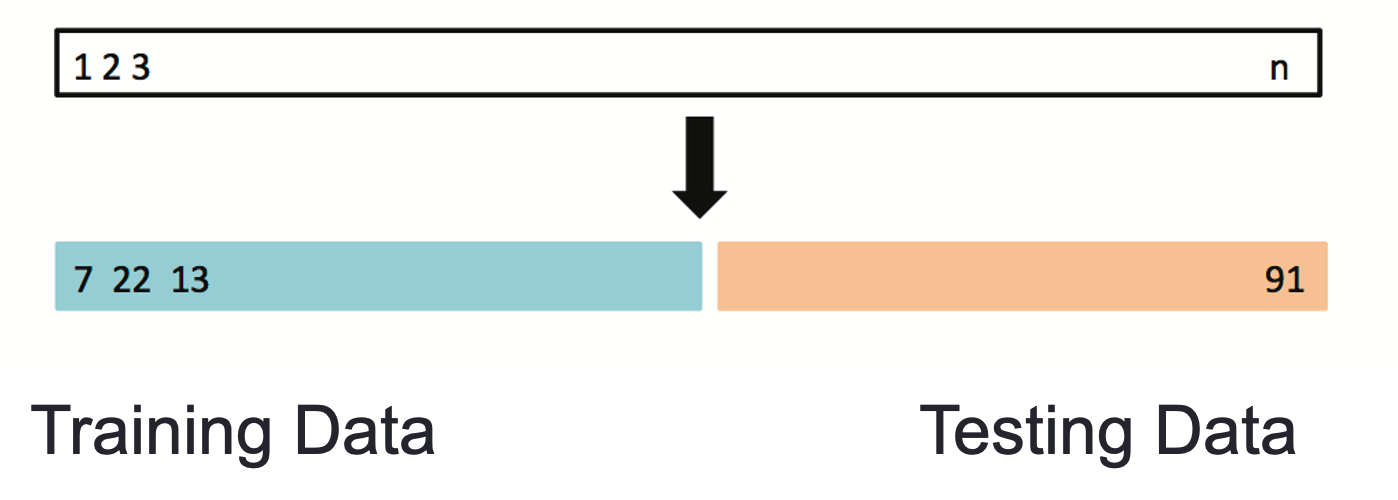
\includegraphics[scale=0.4]{figures/fig51.png}
       \end{figure}

\end{frame}

%----------------------------------------------------------------------%
\begin{frame}[fragile]
\frametitle{Enfoque de conjunto de validación}
\begin{itemize}
\item Modelo $y=f(x) +u$ donde $f$ es un polinomio de grado $p^*$. 
\scriptsize
\item Izquierda: error de predicción en la muestra de prueba para una sola partición
\item Derecha: error de predicción en la muestra de prueba para varias particiones
\item  Hay un monton de variabilidad. (Necesitamos algo mas estable)
\end{itemize}


 \begin{figure}[H] \centering
            \captionsetup{justification=centering}
              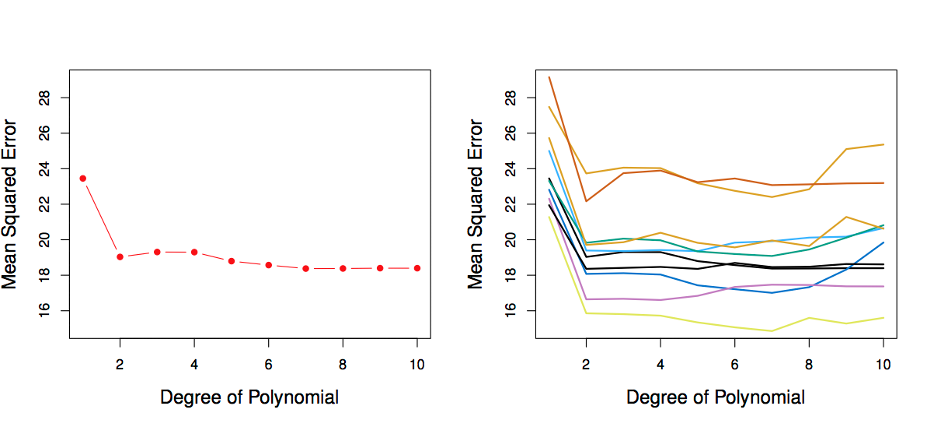
\includegraphics[scale=0.7]{figures/fig52.png}
       \end{figure}
\end{frame}
%----------------------------------------------------------------------%
\begin{frame}[fragile]
\frametitle{Enfoque de conjunto de validación}

\begin{itemize}
  \item Ventajas:
  \medskip
    \begin{itemize}
      \item Simple
      \medskip
      \item Fácil de implementar
      \medskip
    \end{itemize}
  \item Desventajas:
  \medskip
    \begin{itemize}
      \item El MSE de validación (prueba) puede ser altamente variable
      \medskip
      \item  Solo se utiliza un subconjunto de observaciones para ajustar el modelo (datos de entrenamiento). Los métodos estadísticos tienden a funcionar peor cuando se entrenan con pocas observaciones
\end{itemize}
\end{itemize}

\end{frame}
%----------------------------------------------------------------------%
\subsection{LOOCV}
%----------------------------------------------------------------------%
\begin{frame}[fragile]
\frametitle{Leave-One-Out Cross Validation (LOOCV)}

\begin{itemize}
\item Este método es similar al enfoque de validación, pero trata de abordar las desventajas de este último. 
\end{itemize}

 \begin{figure}[H] \centering
            \captionsetup{justification=centering}
              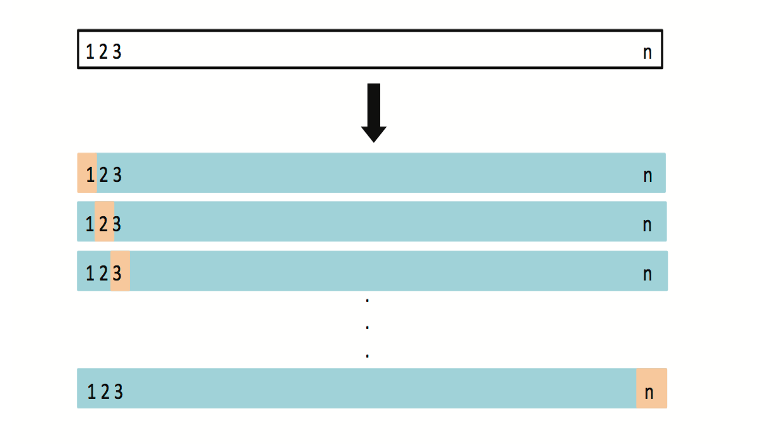
\includegraphics[scale=0.7]{figures/fig53.png}
       \end{figure}


\end{frame}
%----------------------------------------------------------------------%
\subsection{Validación cruzada en K-partes}
%----------------------------------------------------------------------%
\begin{frame}[fragile]
\frametitle{Validación cruzada en K-partes}
\begin{itemize}
\item LOOCV es computacionalmente intensivo, por lo que podemos ejecutar k-fold Cross Validation 
\end{itemize}


 \begin{figure}[H] \centering
            \captionsetup{justification=centering}
              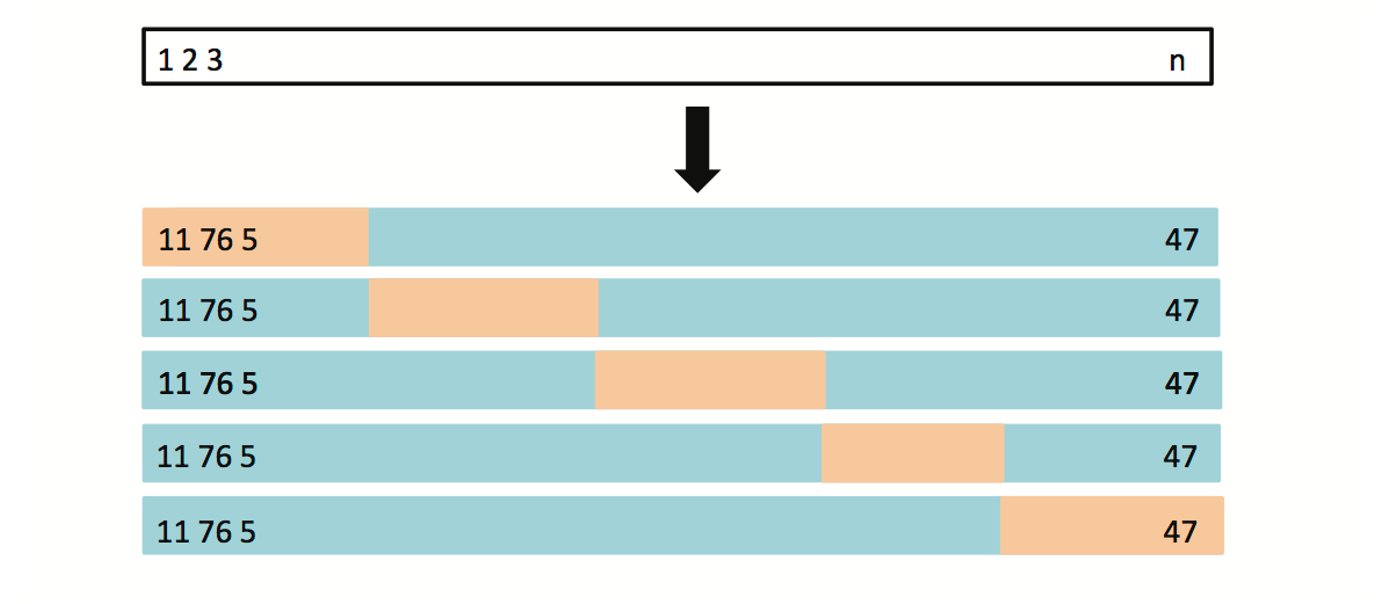
\includegraphics[scale=0.5]{figures/fig55.png}
       \end{figure}



\end{frame}
%----------------------------------------------------------------------%
\begin{frame}[fragile]
\frametitle{Validación cruzada en K-partes}

\begin{itemize}
  \item Dividir los datos en K partes $(N=\sum_{j=1}^K n_j)$
  \medskip
  \item Ajustar el modelo dejando afuera una de las partes (folds)  $\rightarrow$ $f_{-k}(x)$
  \medskip
  \item Calcular el error de predicción en la parte (fold) que dejamos afuera 
  \begin{align}
  \bar{err_j}=MSE_j=\frac{1}{n_j}\sum L(y_j^k,\hat y_{-j})
  \end{align}
  \medskip
\item Promediar

\begin{align}
CV_{(k)}=\frac{1}{k}\sum_{j=1}^k \bar{err_j}= \frac{1}{k}\sum_{j=1}^k MSE_j
\end{align}
\end{itemize}

\end{frame}
%----------------------------------------------------------------------%
\begin{frame}[fragile]
\frametitle{Validación cruzada en K-partes}
\begin{itemize}
  \scriptsize
\item Izquierda: LOOCV  error 
\item Derecha: 10-fold CV 
\item LOOCV es caso especial de k-fold, donde k = n
\item Ambos son estables, pero LOOCV (generalmente) es mas intensivo computacionalmente! 
\end{itemize}

        \begin{figure}[H] \centering
            \captionsetup{justification=centering}
              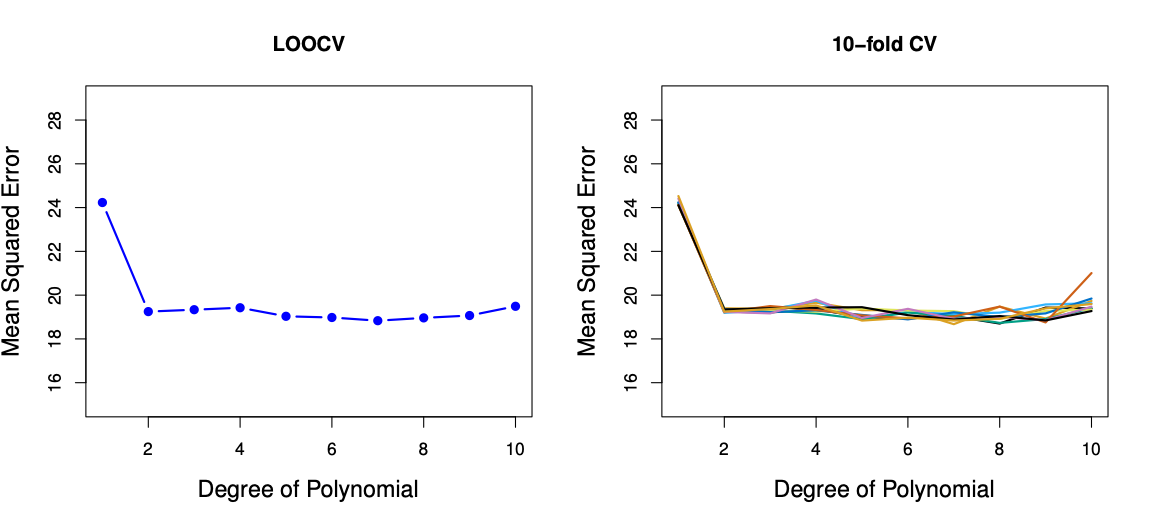
\includegraphics[scale=0.5]{figures/fig54.png}
       \end{figure}
\end{frame}


%----------------------------------------------------------------------%
\begin{frame}[fragile]
\frametitle{Validación cruzada en K-partes para selección de modelos}

\begin{itemize}
  \item Supongamos que $\alpha$ parametriza la complejidad del modelo (en nuestro ejemplo el grado del polinomio)
  \medskip
  \item Primero calculamos el CV error para un grupo de modelos ($\alpha$), y elegimos el minimo

\end{itemize}
\begin{align}
\underset{\alpha}{min} \, CV_{(k)}(\alpha)
\end{align}

        \begin{figure}[H] \centering
            \captionsetup{justification=centering}
              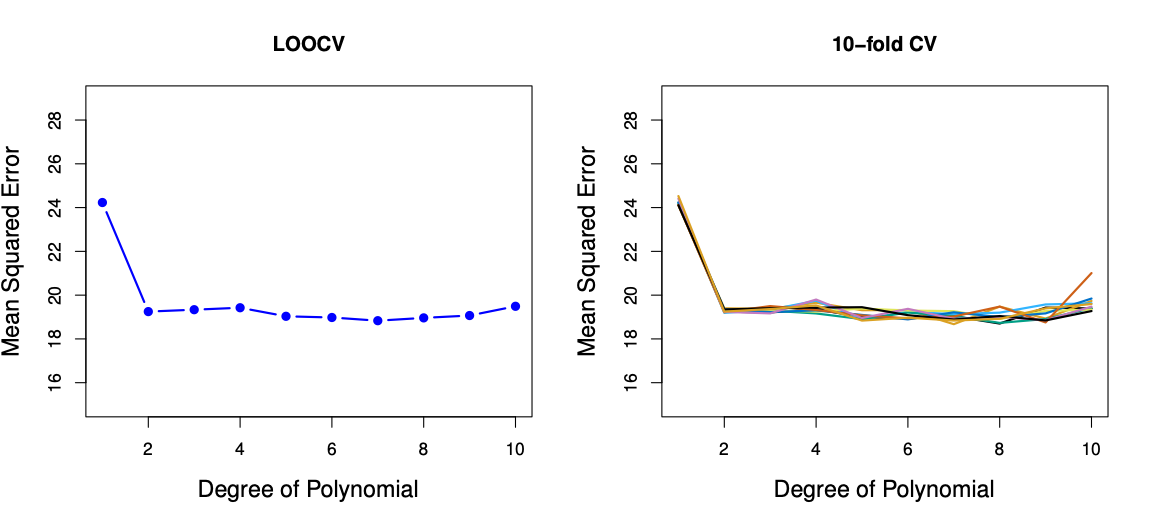
\includegraphics[scale=0.5]{figures/fig54.png}
       \end{figure}

\end{frame}

%----------------------------------------------------------------------%
\begin{frame}[fragile]
\frametitle{Trade-off Sesgo-Varianza para validación cruzada en K-partes}



\begin{itemize}
  \item Sesgo:
  \medskip
    \begin{itemize}
      \item El enfoque del conjunto de validación tiende a sobreestimar el error de predicción en la muestra de prueba (menos datos, peor ajuste)
      \item LOOCV, agrega más datos $ \rightarrow $ menos sesgo 
      \item K-fold un estado intermedio
    \end{itemize}
    \item Varianza:
    \begin{itemize}
      \item LOOCV promediamos los resultados de n modelos ajustados, cada uno está entrenado en un conjunto casi idéntico de observaciones $ \rightarrow $ altamente correlacionado
      \item K partes esta correlación es menor, estamos promediando la salida de k modelo ajustado que están algo menos correlacionados
    \end{itemize}
    \medskip
  \item Por lo tanto, existe un trade-off
  \medskip
    \begin{itemize}
      \item Tendemos a usar k-fold CV con (K = 5 y K = 10)
      \item Se ha demostrado empíricamente que producen estimaciones del error de prediccion que no sufren ni de un sesgo excesivamente alto ni de una varianza muy alta Kohavi (1995)
    \end{itemize}
\end{itemize}

\end{frame}
%----------------------------------------------------------------------%
\begin{frame}
\frametitle{Review \& Next Steps}
  
\begin{itemize} 
    \item Today:
    \medskip
    \begin{itemize} 
         \item Overfit and out of Sample Prediction
         \medskip
         \item Metodos de Resampleo
        \begin{itemize}  
            \item Enfoque de Validación
            \medskip
            \item LOOCV
            \medskip
            \item K-fold Cross-Validation (Validación Cruzada)
      \end{itemize}
    \end{itemize}
    \bigskip  




\end{itemize}
\end{frame}

%----------------------------------------------------------------------%
\section{Further Readings}
%----------------------------------------------------------------------%
\begin{frame}
\frametitle{Further Readings}

\begin{itemize}


  \item Friedman, J., Hastie, T., \& Tibshirani, R. (2001). The elements of statistical learning (Vol. 1, No. 10). New York: Springer series in statistics.
  \medskip
  \item James, G., Witten, D., Hastie, T., \& Tibshirani, R. (2013). An introduction to statistical learning (Vol. 112, p. 18). New York: springer.
  \medskip
    \item Kohavi, R. (1995). A study of cross-validation and bootstrap for accuracy estimation and model selection. In Ijcai (Vol. 14, No. 2, pp. 1137-1145).
  \medskip
  \item Lovelace, R., Nowosad, J., \& Muenchow, J. (2019). Geocomputation with R. CRC Press. (Chapters 2 \& 6)
\end{itemize}

\end{frame}


%----------------------------------------------------------------------%
\section{Break}
\begin{frame}
\frametitle{}

\begin{centering}
\huge
\textcolor{andesred}{Volvemos en 5 min con \texttt{Python} }

\end{centering}

\end{frame}
%----------------------------------------------------------------------%
\section{Continuamos con \texttt{Python y Webscraping}}
%----------------------------------------------------------------------%


%----------------------------------------------------------------------%
\end{document}
